%
% ---------------------------------------------------------------
% Copyright (C) 2012-2018 Gang Li
% ---------------------------------------------------------------
%
% This work is the default powerdot-tuliplab style test file and may be
% distributed and/or modified under the conditions of the LaTeX Project Public
% License, either version 1.3 of this license or (at your option) any later
% version. The latest version of this license is in
% http://www.latex-project.org/lppl.txt and version 1.3 or later is part of all
% distributions of LaTeX version 2003/12/01 or later.
%
% This work has the LPPL maintenance status "maintained".
%
% This Current Maintainer of this work is Gang Li.
%
%

\documentclass[
 size=14pt,
 paper=smartboard,  %a4paper, smartboard, screen
 mode=present, 		%present, handout, print
 display=slides, 	% slidesnotes, notes, slides
 style=tuliplab,  	% TULIP Lab style
 pauseslide,
 fleqn,leqno]{powerdot}


\usepackage{amssymb}
\usepackage{amsmath}
\usepackage{rotating}
\usepackage{graphicx}
\usepackage{boxedminipage}
\usepackage{media9}
\usepackage{rotate}
\usepackage{calc}
\usepackage[absolute]{textpos}
\usepackage{psfrag,overpic}
\usepackage{fouriernc}
\usepackage{pstricks,pst-node,pst-text,pst-3d,pst-grad}
\usepackage{moreverb,epsfig,subfigure}
\usepackage{pstricks}
\usepackage{pstricks-add}
\usepackage{pst-text}
\usepackage{pst-node, pst-tree}
\usepackage{booktabs}
\usepackage{etex}
\usepackage{breqn}
\usepackage{multirow}
\usepackage{gitinfo2}
\usepackage{xcolor}

\usepackage{todonotes}
% \usepackage{pst-rel-points}
\usepackage{animate}
\usepackage{fontawesome}

\usepackage{listings}
\lstset{frameround=fttt,
frame=trBL,
stringstyle=\ttfamily,
backgroundcolor=\color{yellow!20},
basicstyle=\footnotesize\ttfamily}
\lstnewenvironment{code}{
\lstset{frame=single,escapeinside=`',
backgroundcolor=\color{yellow!20},
basicstyle=\footnotesize\ttfamily}
}{}


\usepackage{hyperref}
\hypersetup{ % TODO: PDF meta Data
  pdftitle={Presentation Title},
  pdfauthor={Gang Li},
  pdfpagemode={FullScreen},
  pdfborder={0 0 0}
}


% \usepackage{auto-pst-pdf}
% package to show source code

\definecolor{LightGray}{rgb}{0.9,0.9,0.9}
\newlength{\pixel}\setlength\pixel{0.000714285714\slidewidth}
\setlength{\TPHorizModule}{\slidewidth}
\setlength{\TPVertModule}{\slideheight}
\newcommand\highlight[1]{\fbox{#1}}
\newcommand\icite[1]{{\footnotesize [#1]}}

\newcommand\twotonebox[2]{\fcolorbox{pdcolor2}{pdcolor2}
{#1\vphantom{#2}}\fcolorbox{pdcolor2}{white}{#2\vphantom{#1}}}
\newcommand\twotoneboxo[2]{\fcolorbox{pdcolor2}{pdcolor2}
{#1}\fcolorbox{pdcolor2}{white}{#2}}
\newcommand\vpspace[1]{\vphantom{\vspace{#1}}}
\newcommand\hpspace[1]{\hphantom{\hspace{#1}}}
\newcommand\COMMENT[1]{}

\newcommand\placepos[3]{\hbox to\z@{\kern#1
        \raisebox{-#2}[\z@][\z@]{#3}\hss}\ignorespaces}

\renewcommand{\baselinestretch}{1.2}


\newcommand{\draftnote}[3]{
	\todo[author=#2,color=#1!30,size=\footnotesize]{\textsf{#3}}	}
% TODO: add yourself here:
%
\newcommand{\gangli}[1]{\draftnote{blue}{GLi:}{#1}}
\newcommand{\shaoni}[1]{\draftnote{green}{sn:}{#1}}
\newcommand{\gliMarker}
	{\todo[author=GLi,size=\tiny,inline,color=blue!40]
	{Gang Li has worked up to here.}}
\newcommand{\snMarker}
	{\todo[author=Sn,size=\tiny,inline,color=green!40]
	{Shaoni has worked up to here.}}

%%%%%%%%%%%%%%%%%%%%%%%%%%%%%%%%%%%%%%%%%%%%%%%%%%%%%%%%%%%%%%%%%%%%%%%%
% title
% TODO: Customize to your Own Title, Name, Address
%
\title{Flip 01 and 03 Project Final Presentation}
\author{
Shuxia Lin
\\
\\SouthEast University
}
\date{\gitCommitterDate}


% Customize the setting of slides
\pdsetup{
% TODO: Customize the left footer, and right footer
rf=\href{http://www.tulip.org.au}{
Last Changed by: \textsc{\gitCommitterName}\ \gitVtagn-\gitAbbrevHash\ (\gitAuthorDate)
},
cf={Group Outlying Aspects Mining},
}


\begin{document}

\maketitle

%\begin{slide}{Overview}
%\tableofcontents[content=sections]
%\end{slide}


%%==========================================================================================
%%
\begin{slide}[toc=,bm=]{Overview}
\tableofcontents[content=currentsection,type=1]
\end{slide}
%%
%%==========================================================================================


\section{Problem Definition}


%%==========================================================================================
%%
\begin{slide}[toc=,bm=]{Problem Definition}
\begin{center}
\twotonebox{\rotatebox{90}{Defn}}{\parbox{.86\textwidth}
{Models of emotion are commonly divided into
categorical and dimensional ones.
Dimensional models consider affective states to
be best described relative to a small number of
independent emotional dimensions 
(often two or three): 
Valence 
(a positive-negative scale), 
Arousal 
(a calm–excited scale)
and Dominance 
(perceived degree of control over a situation). 
\begin{itemize}
\item Use Label Distribution Learning
to predict multiple emotion dimension scores for an input text.
Then use the predicted VAD and notational VAD to 
do emotion classification.
\item Use Neural Network to 
do emotion classification.
\end{itemize}
}}
\end{center}

\end{slide}

%%==========================================================================================
%%


\section{Related Work and Challenges}


%%==========================================================================================
%%
\begin{slide}{Related Work - Models of Emotion}
%Related Work - Outlying Aspects Mining


\begin{itemize}
\item
Six Basic Emotions (1992)

\begin{itemize}
\item
anger, happiness, fear, sadness, disgust and surprise
\end{itemize}

\item 
Valence- Arousal-Dominance Model (1994)

\begin{itemize}
	\item 
	Valence (corresponding to the concept of polarity),
	Arousal (a calm-excited scale) and
	Dominance (perceived degree of control in a (social) situation)
\end{itemize}
\begin{center}
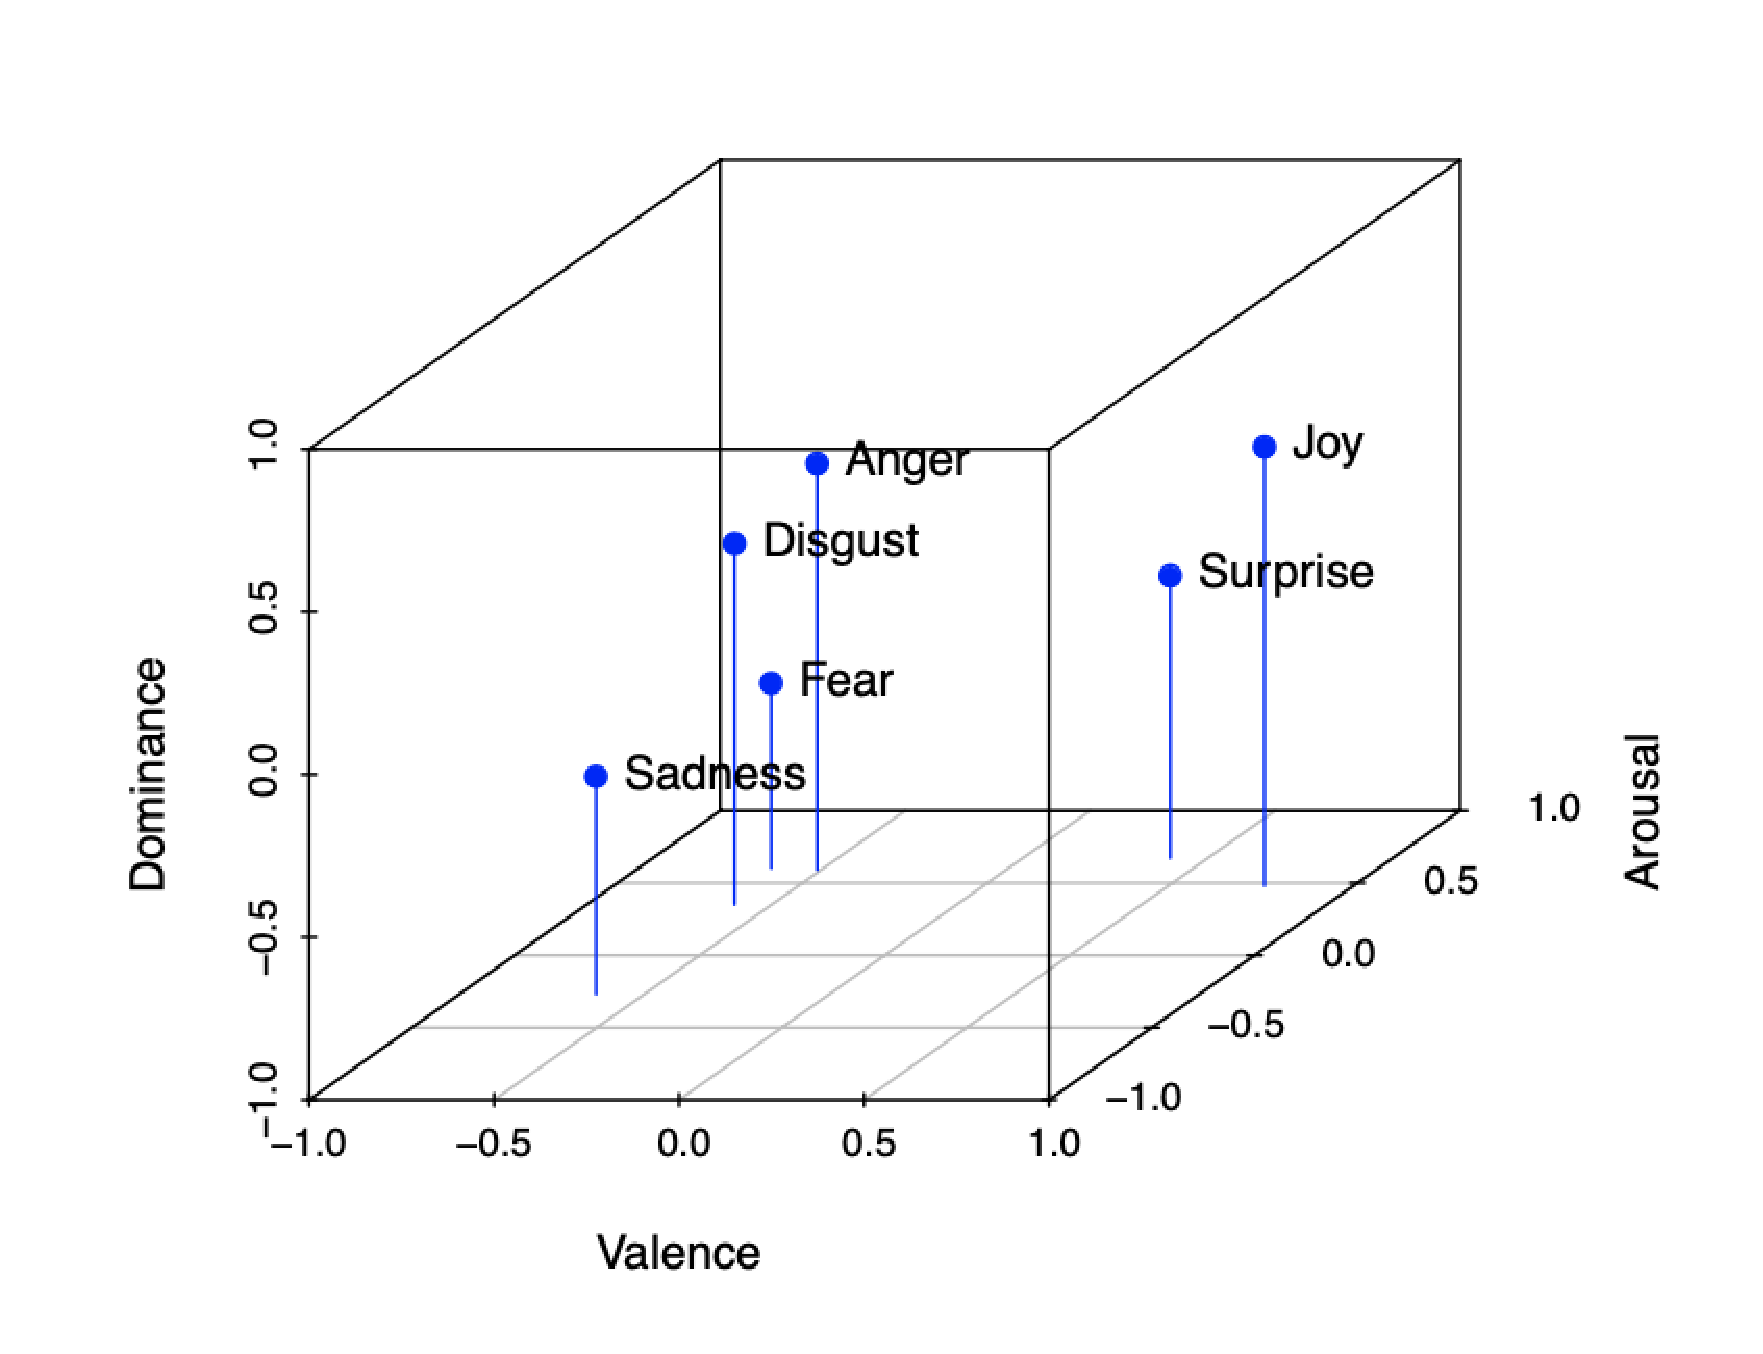
\includegraphics[width=.4\linewidth]{figures/six_emotions_vad.eps}
\end{center}
\end{itemize}

%%==========================================================================================

\end{slide}
%%
%%==========================================================================================


%%==========================================================================================
%%
\begin{slide}{Related Work - Label Distribution Learning}

\begin{itemize}
	\item 
	Formulation of LDL
	
	\begin{itemize}
		\item 
		The training set $ S = \{ ( x_{i} , D_{i} )  \} ˆn_{ i = 1 } $
		\item 
		The label distribution of $ x_{i}  $ is denoted by 
	    $ D_{i} $ = \{ 
	    	$ d ˆ {y_{1}} _{ x_{i} } , 
	    	d ˆ {y_{2}} _{ x_{i} } ,...,
	    	d ˆ {y_{c}} _{ x_{i} }  $ \}
		and 
		$ \sum_{y}  d^y_{x} = 1 $
		\item 
		The goal of LDL is to 
		learn a conditional probability mass function 
		$ p(y|x) $ from $ S $
	\end{itemize}
	
	\item 
	Method of LDL
	
	\begin{itemize}
		\item 
		Suppose $ p(y|x) $  is a parametric model
		 $ p(y|x;{\theta}) $, 
		 where $ \theta $ is the parameter vector. 
		\item 
		Kullback-Leibler divergence	
		
		$ \theta ^{\ast} = 
		 \mathop{\arg\min}\limits_{\theta}
		 \sum\limits_{i}
		 \sum\limits_{j}
		 ( d_{ x_{ i } } ˆ{ y_{ j } }
		 \ln \dfrac{ d_{ x_{ i } } ˆ{ y_{ j } } }{ p( y_{ j } | x_{ i } ;{\theta}) }
		 )$	
		\item 
		Assumes the parametric model 
		$ p(y|x;{\theta}) $ 
		to be the maximum entropy model	
		
		$ p(y|x;{\theta}) = \dfrac{1}{Z}
		\exp ( \sum\limits_{k}
		{\theta}_{y,k} 
		g_{k}( \textbf{x})  ) $ 
		
		where $ Z = \sum _{y}
		\sum_{k}  {\theta}_{y,k}  g_{k}( \textbf{x}) $
		is a normalization factor,
		$ {\theta}_{y,k} $ is an element in \textbf {$\theta$} ,
		and $ g_{k}( \textbf{x}) $ is the \textit{k}-th feature of \textbf{ x }
	\end{itemize}

%%    
\end{itemize}

%%=========================================================================================
\end{slide}
%%
%%==========================================================================================


%%==========================================================================================
%%
\begin{slide}{Challenges }
%Challenges (1)
\begin{itemize}
\item
The output of LDL is the proportion that 
$ y $ accounts for in a full description of $ x $ .
One of the limitation factors is that 
$ \sum_{y}  d^y_{x} = 1 $.
In this problem, the value of 
Valence, Arousal and Dominance 
dimensional emotion scores are labels.
If we just normalize the three values,
after predict we can't get the scores
of the three dimensional emotions.

\bigskip

\item
The lack of large-scale emotion regression corpora in high quality.

\bigskip

\item
Human factors may cause inaccurate labeling of the dataset , 
which may lead to the low accuracy of emotion classification.  

\end{itemize}


\end{slide}
%%
%%==========================================================================================


\section{Data Set}

%%==========================================================================================
%%
\begin{slide}[toc=,bm=]{Data Set}

\begin{itemize}
\item
Emobank contains 10,548 texts annotated with
Valence, Arousal and Dominance 
dimensional emotion scores, 
ranged from 1.0 to 5.0.
\begin{center}
	\begin{tabular}{ c c c c }
		\toprule
		Corpus & Domain  & Raw & Filtered  \\
		\midrule
		SE07 &  news headlines &  1250 &  1192 \\
		\hline
		\multirow{6}{*}{MASC} &  blogs&  1378&  1336\\
		&  essays &  1196 &  1135 \\
		&  fiction &  2893 &  2753 \\
		&  letters &  1479 &  1413 \\
		& newspapers & 1381 & 1314 \\
		& traval guides & 971 & 919 \\
		\bottomrule
	\end{tabular}
\end{center}

\item 
SE07 is  annotated according to 
Ekman’s six Basic Emotion 
on a [0,100] scale, respectively.

\end{itemize}

\end{slide}
%%
%%==========================================================================================

\section{Method}


%%==========================================================================================
%
\begin{slide}{Dimensional Emotion Distribution Learning Algorithm}

\begin{itemize}
	\item Model
	
	\begin{itemize}
		\item 
		The training set $ S = \{ ( x_{i} , D_{i} )  \} ˆn_{ i = 1 } $
		\item 
		The label distribution of $ x_{i}  $ is denoted by 
		$ D_{i} $ = \{ 
		$ d ˆ {y_{v}} _{ x_{i} } , 
		d ˆ {y_{a}} _{ x_{i} } ,
		d ˆ {y_{d}} _{ x_{i} } ,
		d ˆ {y_{n}} _{ x_{i} }  $ \}
		
		where $ d ˆ {y_{v}} _{ x_{i} }  = \dfrac{scoreˆ{v}_{ x_{i} }} {15} $ , 
		 $ d ˆ {y_{a}} _{ x_{i} }  = \dfrac{scoreˆ{a}_{ x_{i} }} {15} $ ,
		  $d ˆ {y_{a}} _{ x_{i} }= \dfrac{scoreˆ{d}_{ x_{i} }}{15} $ 
		  and $ y_{n} = 1 - y_{v}  - y_{a} - y_{d} $
	\end{itemize}

	\item 
	Proof
	
	\begin{itemize}
		\item 
		Assume $ T(\theta) =  \mathop{\arg\min}\limits_{\theta}
		\sum\limits_{i}
		\sum\limits_{j}
		( d_{ x_{ i } } ˆ{ y_{ j } }
		\ln \dfrac{ d_{ x_{ i } } ˆ{ y_{ j } } }{ p( y_{ j } | x_{ i } ;{\theta}) } $,
		for each step, it updates the current estimate of the parameters 
		\textbf{$\theta$} to \textbf{ $\theta + \delta$},
		where \textbf{$ \delta $} minimizes a lower bound to the change in likelihood
		$ T(\theta + \delta) - T(\theta) = \sum\limits_{ij} 
		 d_{ x_{ i } } ˆ{ y_{ j } } (
		 \ln p( y_{ j } | x_{ i } ;{\theta}) -
		 \ln p( y_{ j } | x_{ i } ;{\theta + \delta}) )$
		 
		 \item 
		 For rmse,
		 $ \mathop{\min}\sum\limits_{ij}
		  (d_{ x_{ i } } ˆ{ y_{ j } }  - 
		  p( y_{ j } | x_{ i } ;{\theta}))ˆ2$
		  is equal to 
		  $ R(\theta) = \mathop{\min} \sum\limits_{ij}
		  |d_{ x_{ i } } ˆ{ y_{ j } }  - 
		  p( y_{ j } | x_{ i } ;{\theta})| $,
		  and for each update,
		  $ R(\theta + \delta) - R(\theta) 
		  \leq  
		  \sum\limits_{ij} |
		  d_{ x_{ i } } ˆ{ y_{ j } }  - 
		  p( y_{ j } | x_{ i } ;{\theta + \delta}) - 
		  (d_{ x_{ i } } ˆ{ y_{ j } }  - 
		  p( y_{ j } | x_{ i } ;{\theta})) | =
		  \sum\limits_{ij}
		  | \ln p( y_{ j } | x_{ i } ;{\theta}) -
		  \ln p( y_{ j } | x_{ i } ;{\theta + \delta}) |$
		 
	\end{itemize}
\end{itemize}

\end{slide}
%%
%%==========================================================================================

\begin{slide}{TextCNN}
	
The textCNN model mainly uses 
a one-dimensional convolutional layer and 
a max-over-time pooling layer. 
Assume that 
the input text sequence consists of $ n $ words, 
and each word is represented by 
a $ d  $dimensional word vector. 
Then the width of the input sample is$  n $, 
the height is 1, 
and the number of input channels is $ d $. 
The calculation of textCNN is mainly divided into the following steps.

\begin{itemize}
	\item 
	Define multiple one-dimensional convolution kernels, 
	and use these convolution kernels to 
	perform convolution calculations on the inputs. 
	\item 
	All the channels of the output are individually pooled 
	in max-over-time pooling, 
	and the pooled output values of 
	these channels are connected into a vector.
	\item 
	The fully connected layer transforms 
	the connected vectors into outputs for each class. 
	This step can use the dropout layer to deal with overfitting.
\end{itemize}

\end{slide}
%%
%%==========================================================================================

\begin{slide}[toc=,bm=]{TextCNN}
	
\begin{center}
	\includegraphics[width=.7\linewidth]{figures/textCNN.eps}
\end{center}	

\end{slide}


%%
%%==========================================================================================

\begin{slide}{LSTM}
In the code I implement 
\begin{itemize}
	\item 
	 the Embedding instance is the embedding layer
	 \item 
	 the LSTM instance is the hidden layer of sequence encoding
	 \item 
	 the Linear instance is the output layer that generates the classification results
\end{itemize}

\bigskip

\begin{figure}
	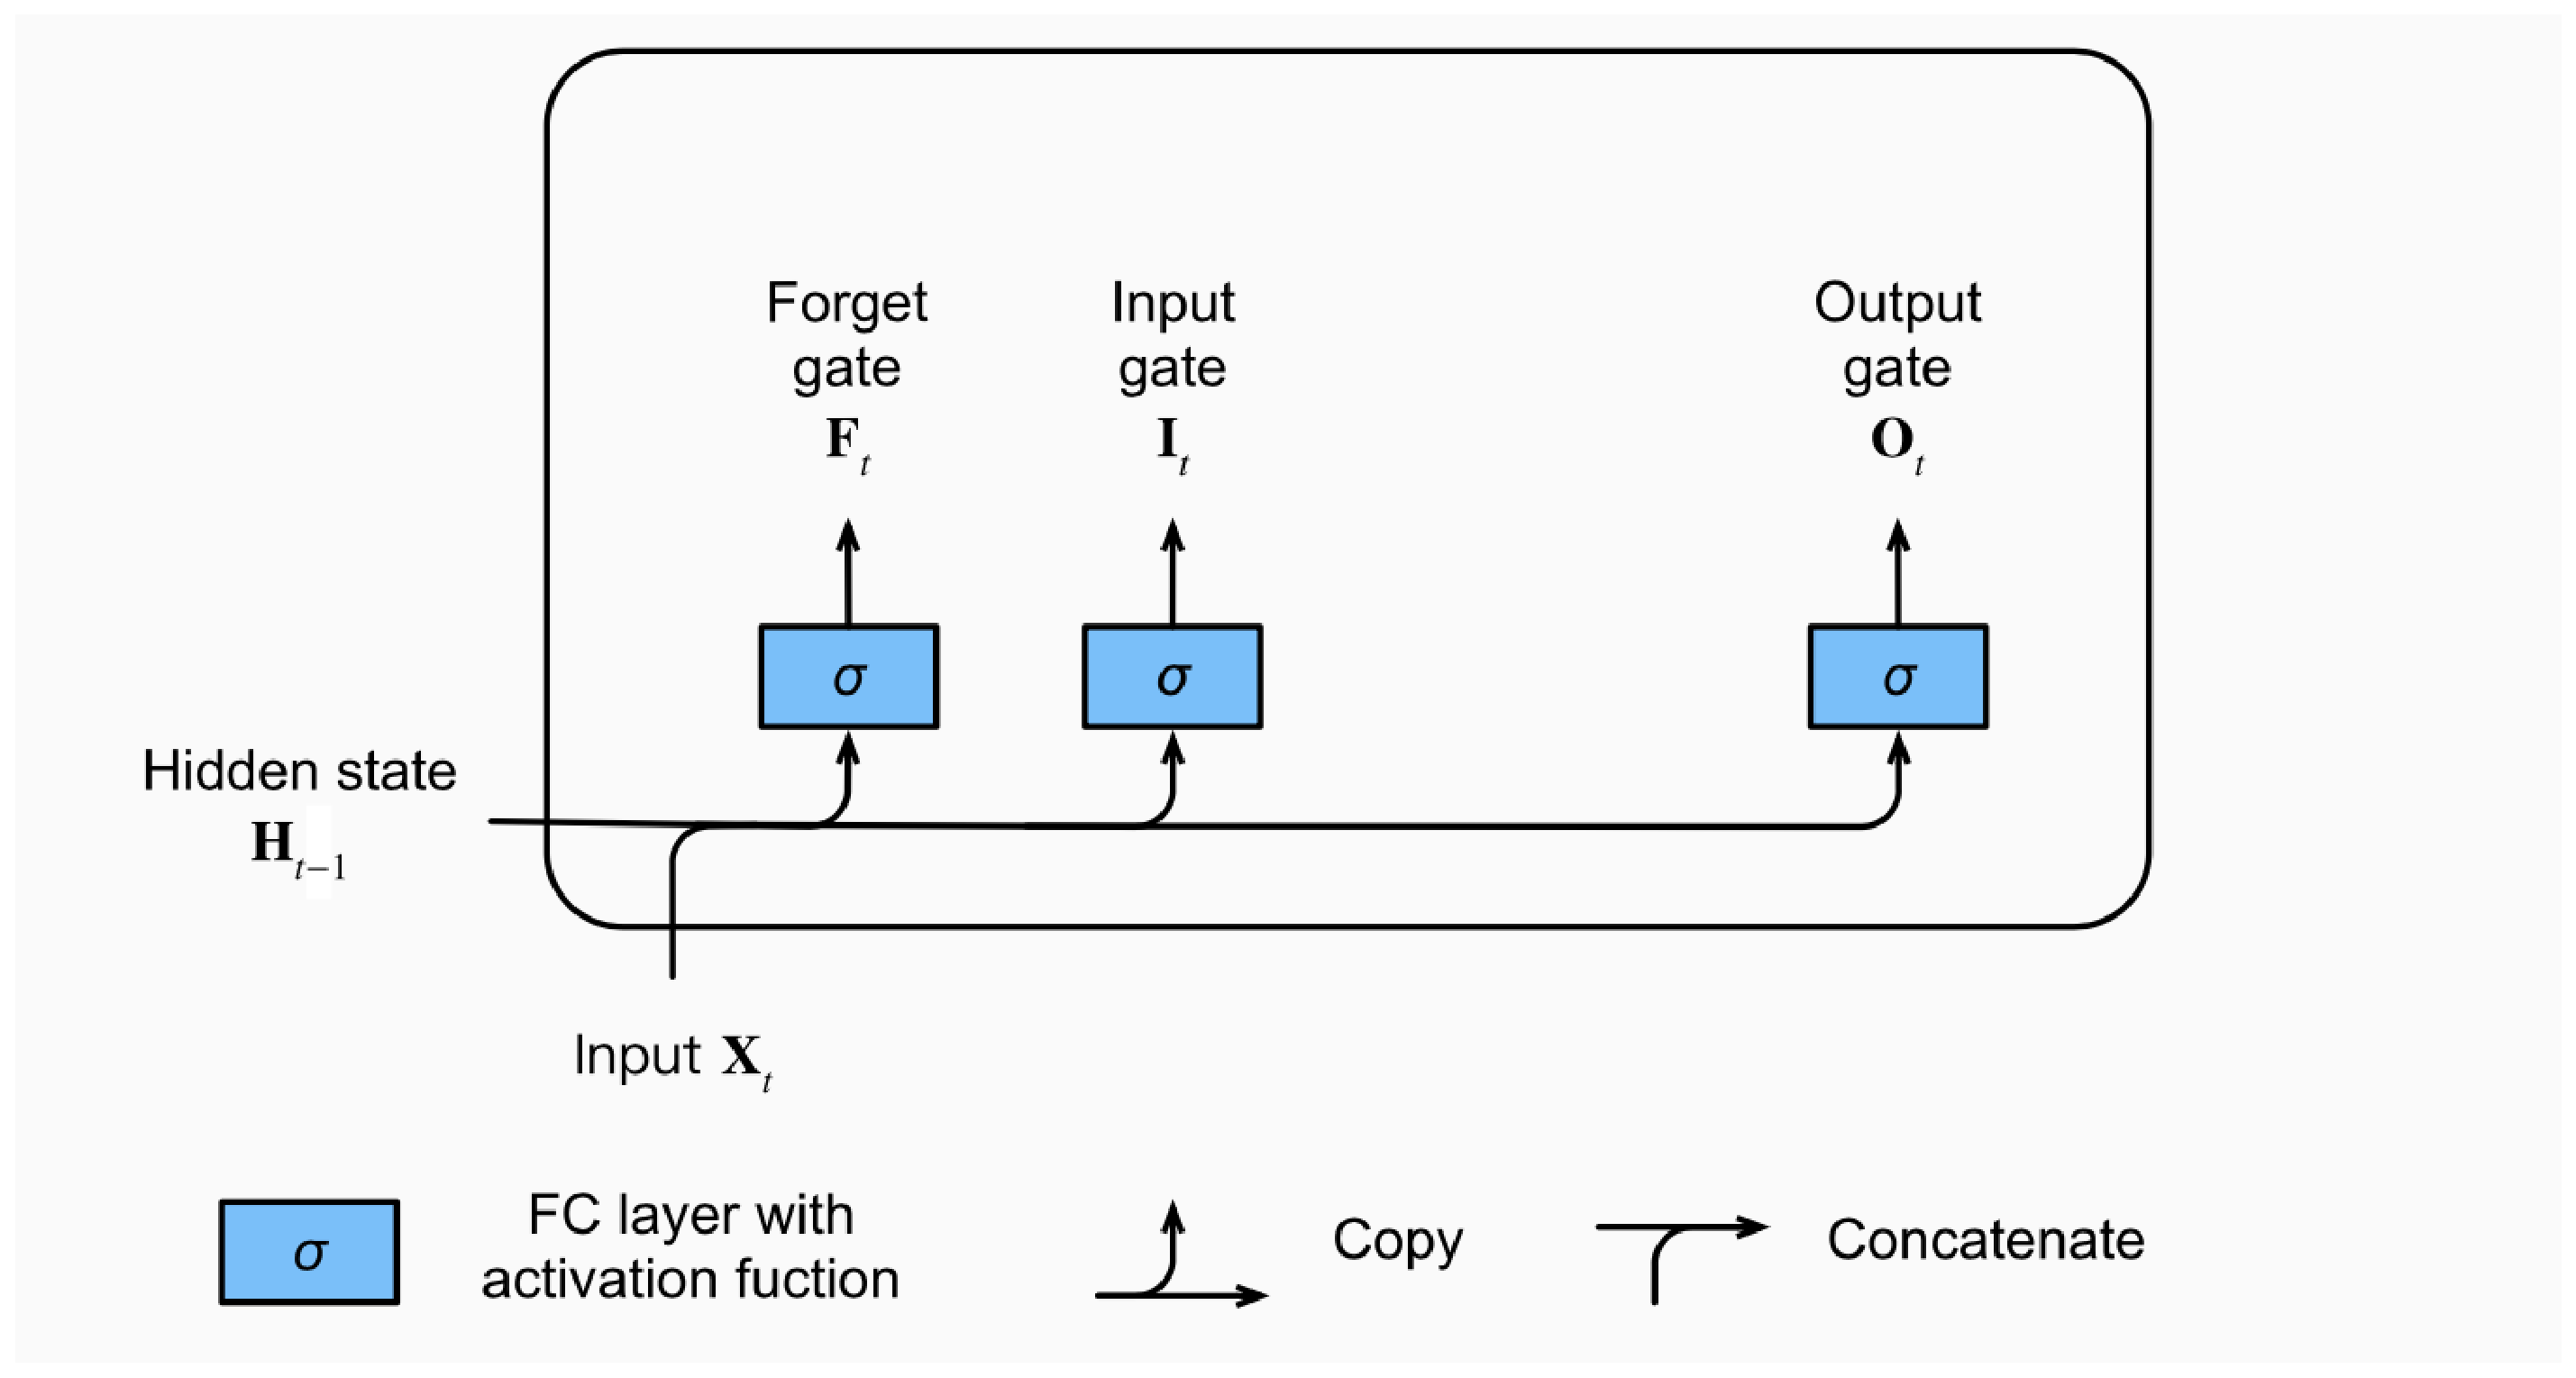
\includegraphics[width=.5\linewidth]{figures/lstm_en.eps}
	\caption{Calculation of input, forget, and output gates in an LSTM}
\end{figure}


\end{slide}

%%
%%==========================================================================================


\section{Experiment}

%%==========================================================================================
%%
\begin{slide}{Experiment One}
%Step One - Group Feature Extraction}
\begin{itemize}
\item
Data Processing

\begin{itemize}
	\item 
	Use Bert to train the sentence encoding/embedding
	of Emobank corpus, that is the feature vectors $ x_{i} $
	\item 
	Transform the scores of Valence, Arousal and Dominance 
	dimensional emotion into 
	the label distribution 
	$ D_{i} $ = \{ 
	$ d ˆ {y_{v}} _{ x_{i} } , 
	d ˆ {y_{a}} _{ x_{i} } ,
	d ˆ {y_{d}} _{ x_{i} } ,
	d ˆ {y_{n}} _{ x_{i} }  $ \}
\end{itemize}

\item 
Predict the scores of 
Valence, Arousal and Dominance dimensional emotion
through the EDLD
for the sentences in the SE07 corpus.

\item 
New Data Set

\begin{itemize}
	\item 
	DATASET_1 : predicted VAD is the features and 
	the emotion categories corresponding to 
	the max scales of the sentences in SE07.
	\item 
	DATASET_2 : Annotated VAD is the features and 
	the emotion categories corresponding to 
	the max scales of the sentences in SE07.
\end{itemize}

\item 
Algorithm

\begin{itemize}
	\item DecisionTree, KNeighbors, LogisticRegression and so on.
	
\end{itemize}
\end{itemize}

\end{slide}
%%
%%==========================================================================================

\begin{slide}{Experiment Two }
%Step Two - Outlying Degree Scoring
\bigskip

\begin{itemize}

\item 
Load data
\item 
Text Preprocessing

\begin{itemize}
	\item 
	Tokenization : Split strings into tokens
	\item 
	Vocabulary : Build a vocabulary for these tokens to map them into numerical indices.
	\item 
	
\end{itemize}

\item 
Using a TextCNN or LSTM Model

\item 
Loading Pre-trained Word Vectors

\item 
Training and Evaluating the Model

\end{itemize}

\end{slide}
%%
%%==========================================================================================



\section{Evaluation Results}


%%==========================================================================================
%%
\begin{slide}[toc=,bm=]{Evaluation}

\begin{center}
\begin{itemize}

\item
\smallskip
\large
{$Accuracy = \frac{P}{T}$ \\
P: Identified outlying aspects \\

T: Real outlying aspects}

\end{itemize}
\end{center}

\end{slide}
%%
%%==========================================================================================


\begin{slide}{Results}

\begin{table}[tb]
\setlength{\abovecaptionskip}{0pt}
\setlength{\belowcaptionskip}{10pt}
\centering
\caption{The experiment result on synthetic dataset}

\begin{tabular}{ c | c | c | c }
\toprule
  % after \\: \hline or \cline{col1-col2} \cline{col3-col4} ...
  Method     &  Truth Outlying Aspects    & Identified Aspects & Accuracy      \\
\midrule
  GOAM       &  $\{F_1\}$, $\{F_2F_4\}$   &  $\{F_1\}$, $\{F_2F_4\}$    & 100\%    \\

Arithmetic Mean based OAM &  $\{F_1\}$, $\{F_2F_4\}$   &  $\{F_4\}$, $\{F_2\}$    &  0\% \\

Median based OAM &  $\{F_1\}$, $\{F_2F_4\}$   &  $\{F_2\}$, $\{F_4\}$    &           0\% \\
\bottomrule
\end{tabular}
\end{table}

\end{slide}
%%
%%==========================================================================================


\section{Conclusion}

%%==========================================================================================
%%
\begin{slide}[toc=,bm=]{Conclusion}
\begin{itemize}
\item
\smallskip
Formalize the problem of \emph{Group Outlying Aspects Mining} by
extending outlying aspects mining;

\item
\smallskip
Propose a novel method \textcolor{orange}{GOAM algorithm} to solve the
\emph{Group Outlying Aspects Mining} problem;

\item
\smallskip
Utilize the pruning strategies to reduce time complexity.

\end{itemize}

%%==========================================================================================
\begin{note}
In conclusion,
we firstly formalized the problem of
group outlying aspects mining,

Then proposed a novel method GOAM algorithm to address the problem of
group outlying aspects mining,
and the proposed method use pruning to reduce time complexity
while identifying the suitable set of outlying features for the interested group.

Thank you and any question?
\end{note}
%%==========================================================================================

\end{slide}
%%
%%==========================================================================================


%%==========================================================================================
%
\begin{slide}[toc=,bm=]{Questions?}
\begin{center}
\begin{figure}
    \animategraphics[autoplay, loop, height=0.4\textheight]{5}{figures//gif//question//q_}{1}{30}
\end{figure}
\end{center}
\end{slide}
%%
%%==========================================================================================


%%==========================================================================================
% TODO: Contact Page
\begin{wideslide}[toc=,bm=]{Contact Information}
\centering
\vspace{\stretch{1}}
\twocolumn[
lcolwidth=0.35\linewidth,
rcolwidth=0.65\linewidth
]
{
% \centerline{
\includegraphics[scale=.2]{tulip-logo.eps}}
}
{
\vspace{\stretch{1}}
Associate Professor Gang Li\\
School of Information Technology\\
Deakin University, Australia
\begin{description}
 \item[\textcolor{orange}{\faEnvelope}] \href{mailto:gangli@tulip.org.au}
 {\textsc{\footnotesize{gangli@tulip.org.au}}}

 \item[\textcolor{orange}{\faHome}] \href{http://www.tulip.org.au}
 {\textsc{\footnotesize{Team for Universal Learning and Intelligent Processing}}}
\end{description}
}
\vspace{\stretch{1}}
\end{wideslide}

\end{document}

\endinput
